%% ═══════════════════════════════════════════════════════════════════════════
\chapter{Neural Network Pruning}
\label{chap:neural_network_pruning}
%% ═══════════════════════════════════════════════════════════════════════════

\section{Introduction}

Within the broader framework established in Chapter~\ref{chap:foundations}, pruning may
be understood as a constrained simplification of a trained network. The
optimization perspective determines how pruning error is measured, the
architectural decomposition of neural and Transformer blocks determines what
may be removed, and the deployment metrics determine whether sparsity produces
only nominal compression or an actual computational gain.

Pruning is a central compression mechanism for deep neural networks. Its
objective is to reduce the number of active parameters or executable units
while preserving the predictive behaviour of the reference model. It modifies
the \emph{effective topology} of the model by removing weights, channels,
heads, layers, or other structural components. Pruning is therefore both a
compression problem and an architectural selection problem.

The relevance of pruning follows from the over-parameterised nature of modern
neural networks. Large models often contain substantial redundancy distributed
unevenly across layers and parameter groups. In practice, pruning is governed
by two coupled design variables: the criterion used to identify removable
units and the allocation rule used to distribute the retained budget across
layers or structures.

These questions become especially important in Transformers, where storage cost,
memory traffic, and latency depend not only on parameter count but also on the
structure of attention and feed-forward blocks.

Over-parameterisation reflects the empirical observation that very wide
networks often generalise better than the minimum architecture required to fit
the training data. The additional parameters support optimization and
representation learning, but many contribute only marginally to the final
function. Pruning exploits this redundancy by identifying units whose removal
causes limited degradation.

Current model scales make pruning operationally relevant. The representative
counts below follow the corresponding architecture reports for ResNet-50,
BERT, GPT-2, and LLaMA-2; GPT-4 is included only to indicate that frontier
closed models have undisclosed parameter counts and architectures
\cite{He2016,devlin2019bert,radford2019language,touvron2023llama2,achiam2023gpt}.

Table~\ref{tab:model_sizes} summarises the parameter counts and memory footprints of these models in FP32 and FP16.  The memory footprints are computed as follows:
\begin{align}
	\text{Memory}_{\mathrm{FP32}} &= P \times 4\,\text{bytes}, \\
	\text{Memory}_{\mathrm{FP16}} &= P \times 2\,\text{bytes}.
\end{align}
and represent the storage required for the model parameters alone, excluding activations, optimizer states, or other overheads.
\begin{table}[H]
	\centering
	\caption{Parameter counts and memory footprints for selected modern models.
		FP16 storage assumes 2 bytes per parameter.}
	\label{tab:model_sizes}
	\small
	\renewcommand{\arraystretch}{1.3}
	\begin{tabularx}{\textwidth}{lrrrX}
		\toprule
		\textbf{Model} & \textbf{Params} & \textbf{FP32 (GB)} & \textbf{FP16 (GB)}
		& \textbf{Notes} \\
		\midrule
		ResNet-50          & 25.6 M  & 0.10 & 0.05 & Image classification \\
		BERT-Base          & 110 M   & 0.44 & 0.22 & Encoder-only LM \\
		GPT-2 (XL)        & 1.56 B  & 6.24 & 3.12 & Auto-regressive LM \\
		LLaMA-2 (7B)      & 6.74 B  & 26.9 & 13.5 & Open-weight LLM \\
		LLaMA-2 (70B)     & 68.9 B  & 275  & 138  & Requires multiple GPUs \\
		GPT-4             & --       & --         & --         & Parameters not publicly disclosed \\
		\bottomrule
	\end{tabularx}
\end{table}

Even at 50\% unstructured sparsity, a 70B-parameter model still demands roughly
70\,GB of storage in FP16. Practical deployment therefore requires either
higher sparsity ratios or removal patterns that translate into actual execution
gains on the target hardware.

%% ─────────────────────────────────────────────────────────────────────────
\section{Theoretical Framework of Pruning}
%% ─────────────────────────────────────────────────────────────────────────

Since pruning is a constrained optimisation problem, its theoretical analysis relies on tools from combinatorial optimisation, Taylor expansions, and information theory.  The following sections formalise the pruning problem, characterise the loss change induced by pruning, and review foundational criteria such as Optimal Brain Damage and Optimal Brain Surgeon.
\subsection{Formal Problem Formulation}

Let a neural network be denoted by $f(x;\Theta)$, where
$\Theta = \{\theta_i\}_{i=1}^{P}$ is the full parameter set of cardinality
$P$.  Pruning introduces a binary \emph{mask} variable $M$ that determines
which parameters or groups remain active.  For unstructured pruning, the
masked model can be written as

\begin{equation}
	f_{\mathrm{pr}}(x;\Theta,M) = f(x; M \odot \Theta),
	\label{eq:masked_model}
\end{equation}

where $M \in \{0,1\}^{P}$ and $\odot$ denotes the Hadamard (elementwise)
product.  When $M_i = 0$, parameter $\theta_i$ is zeroed out and removed
from the effective computation graph.
%
%\begin{definition}{Pruning Problem}{}
%	Given a loss function $\mathcal{L}$, a target density $\kappa \in (0,1]$,
%	and a parameter set $\Theta$, the pruning problem is
%	\begin{equation}
%		\min_{\Theta, M}\; \mathcal{L}(M \odot \Theta)
%		\quad
%		\text{subject to}
%		\quad
%		\frac{\norm{M}_0}{P} \le \kappa,
%		\label{eq:constrained}
%	\end{equation}
%	where $\norm{\cdot}_0$ counts the number of nonzero entries (or active
%	groups).  The equivalent Lagrangian relaxation is
%	\begin{equation}
%		\min_{\Theta, M}\; \mathcal{L}(M \odot \Theta) + \lambda\,\Omega(M),
%		\label{eq:regularised}
%	\end{equation}
%	where $\Omega(M)$ penalises model complexity, hardware cost, or sparsity.
%\end{definition}

To give a robust definition, we need to specify the loss function $\mathcal{L}$, the pruning budget $\kappa$, and the structure of the mask $M$.  The loss is typically the empirical risk on a validation set, which serves as a proxy for generalisation performance.  The budget $\kappa$ is a user-defined hyperparameter that determines the target density of the pruned model.  The mask structure depends on the pruning regime (unstructured, semi-structured, or structured) and defines the feasible set of pruned models.
Given these definitions and constraints, the pruning problem can be formalised as a constrained optimisation problem definied by equation \eqref{eq:constrained} or its Lagrangian relaxation in \eqref{eq:regularised}.
\begin{equation}
\min_{\Theta, M}\; \mathcal{L}(M \odot \Theta)
\quad
\text{subject to}
\quad
\frac{\norm{M}_0}{P} \le \kappa,
\label{eq:constrained}
\end{equation}
\begin{equation}
\min_{\Theta, M}\; \mathcal{L}(M \odot \Theta) + \lambda\,\Omega(M),
\label{eq:regularised}
\end{equation}

Where $\Omega(M)$ is a regularisation term that penalises model complexity, hardware cost, or sparsity, and $\lambda$ is a hyperparameter that controls the trade-off between loss minimisation and model compression.

\medskip
%The constraint \eqref{eq:constrained} reveals the fundamental difficulty:
%even with $\Theta$ fixed, finding the optimal mask $M^*$ is an NP-hard
%combinatorial search over $\{0,1\}^P$.  For a network with $P = 7 \times 10^9$
%parameters (LLaMA-2-7B), the feasible set is astronomically large; exhaustive
%search is completely infeasible.  Practical methods therefore rely on
%\emph{saliency surrogates}, \emph{differentiable relaxations}, or
%\emph{greedy heuristics}.

The constraint \eqref{eq:constrained} reveals the fundamental difficulty of pruning: even with $\Theta$ fixed, finding the optimal mask $M^*$ is an NP-hard combinatorial search over $\{0,1\}^P$ ~\cite{blumensath2008iterative}. For a network with $P = 7 \times 10^9$ parameters (LLaMA-2-7B), the feasible set is astronomically large; exhaustive search is completely infeasible. Practical methods therefore rely on saliency surrogates, differentiable relaxations, or greedy heuristics to find an approximate solution.

\subsection{Taylor Expansion Analysis of Pruning Loss}

The impact of pruning on the loss function can be rigorously characterised
through a Taylor expansion.  Let $\Theta^*$ be the trained (reference) weights
and let $\delta\Theta = M \odot \Theta^* - \Theta^*$ be the perturbation
induced by masking.  Expanding the loss around $\Theta^*$:

\begin{equation}
	\Delta\mathcal{L} = \mathcal{L}(\Theta^* + \delta\Theta)
	- \mathcal{L}(\Theta^*)
	\approx
	\underbrace{\nabla\mathcal{L}(\Theta^*)^\top \delta\Theta}_{\text{1st order}}
	+
	\frac{1}{2}\,\underbrace{\delta\Theta^\top H(\Theta^*)\,\delta\Theta}_{\text{2nd order}}
	+ \mathcal{O}(\norm{\delta\Theta}^3),
	\label{eq:taylor}
\end{equation}

where $H(\Theta^*) \in \R^{P \times P}$ is the Hessian of the loss evaluated
at $\Theta^*$.  This single expression motivates the entire family of pruning
criterias represented in Table~\ref{tab:criterion_families}.

\begin{table}[H]
	\centering
	\caption{Pruning criterion families derived from the Taylor expansion.}
	\label{tab:criterion_families}
	\renewcommand{\arraystretch}{1.5}
	\begin{tabularx}{\textwidth}{llXl}
		\toprule
		\textbf{Order} & \textbf{Family} & \textbf{Approximation}
		& \textbf{Cost} \\
		\midrule
		0th & Magnitude & $\Delta\mathcal{L} \approx 0$; use $|\theta_i|$ as proxy.
		& $O(P)$ \\[2pt]
		1st & Gradient-based &
		$\Delta\mathcal{L} \approx \nabla\mathcal{L}(\Theta^*)^\top\delta\Theta$;
		use $\bigl|\tfrac{\partial\mathcal{L}}{\partial\theta_i}\theta_i\bigr|$.
		& $O(P)$ + 1 backward pass \\[2pt]
		2nd (diag.) & OBD-style &
		$\Delta\mathcal{L} \approx \frac{1}{2} H_{ii}\theta_i^2$; diagonal
		Hessian approximation.
		& $O(P)$ + Hessian diag.\ \\[2pt]
		2nd (block) & OBS / SparseGPT &
		Optimal weight update $\delta W$ alongside mask;
		per-layer blockwise Hessian inversion.
		& $O(d^3)$ per layer\\
		\bottomrule
	\end{tabularx}
\end{table}

At a stationary point where $\nabla\mathcal{L}(\Theta^*) \approx 0$ (fully
converged training), the first-order term vanishes and the second-order
term dominates, making curvature the decisive quantity.

\subsection{Optimal Brain Damage and Optimal Brain Surgeon}

Two classical second-order formulations remain foundational to later pruning
methods.

\paragraph{Optimal Brain Damage (OBD, LeCun et al.\ 1989.)}
OBD assumes a diagonal Hessian ($H \approx \diag(H_{11}, \ldots, H_{PP})$)
and no weight update after deletion.  Under these assumptions the saliency of
parameter $\theta_i$ is \cite{lecun1989optimal}

\begin{equation}
	S_i^{\mathrm{OBD}} = \frac{1}{2}\, H_{ii}\,\theta_i^2.
	\label{eq:obd}
\end{equation}

The diagonal approximation decouples parameters and permits individual
ranking.  However, it underestimates the true loss change whenever Hessian
off-diagonal entries are significant.

\paragraph{Optimal Brain Surgeon (OBS, Hassibi \& Stork 1993.)}
OBS removes a scalar parameter $q$ while jointly updating the remaining
weights $\delta\Theta^*$ to compensate, yielding the exact second-order
optimal re-fitting \cite{hassibi1993second}:

\begin{equation}
	\delta\Theta^* = -\frac{\theta_q}{[H^{-1}]_{qq}}\, H^{-1} e_q,
	\qquad
	\Delta\mathcal{L}_q = \frac{\theta_q^2}{2\,[H^{-1}]_{qq}},
	\label{eq:obs}
\end{equation}

where $e_q$ is the $q$-th standard basis vector and $[H^{-1}]_{qq}$ is the
$(q,q)$ element of the inverse Hessian.

OBS achieves strictly lower loss
increase than OBD, but inverting $H \in \R^{P \times P}$ is prohibitive at
scale.  Modern methods such as SparseGPT and GPTQ adapt OBS-style local
reconstruction to the blockwise, per-layer setting to make it tractable
\cite{frantar2023sparsegpt,frantar2022gptq}.

\subsection{Density, Sparsity, and Effective Topology}
	Let $N_\mathrm{act}$ denote the number of active (nonzero) parameters.
	The \emph{density} and \emph{sparsity} of a pruned network are defined by the equation ~\eqref{eq:density_sparsity}:
	\begin{equation}
		\rho = \frac{N_\mathrm{act}}{P}, \qquad s = 1 - \rho.
		\label{eq:density_sparsity}
	\end{equation}

\medskip
Identical values of $s$ can correspond to radically different models.
Consider a $10^6$-parameter network with $s = 0.90$:

\begin{itemize}[nosep]
	\item If the 10\% remaining weights are \emph{uniformly distributed} across
	layers, every matrix operation remains dense at reduced size.
	\item If the 10\% remaining weights are \emph{concentrated in two layers},
	those layers are effectively unpruned while eight others are almost
	dead.
	\item If the pattern is \emph{irregular}, hardware cannot exploit the zeros
	without sparse-format overhead.
\end{itemize}

Sparsity alone is therefore insufficient to characterize a pruned network.
%
%\subsection{Computations of a Pruned Neural Network}
%
%\paragraph{Dense baseline.}
%Consider a linear layer with weight matrix $W \in \R^{m \times n}$, bias
%$b \in \R^m$, and input $x \in \R^n$:
%\begin{equation}
%	h = Wx + b.
%	\label{eq:dense_linear}
%\end{equation}
%This requires exactly $mn$ multiply-accumulate operations (MACs) and $mn$
%stored parameters.
%
%\paragraph{Unstructured sparsity.}
%Under mask $M \in \{0,1\}^{m \times n}$:
%\begin{equation}
%	\hat{h} = (M \odot W)x + b.
%	\label{eq:sparse_linear}
%\end{equation}
%Theoretical MACs drop to $\rho\,mn$ where $\rho = \norm{M}_0 / (mn)$, but
%practical speedup requires a sparse execution engine that skips the zero
%multiplications.
%
%\paragraph{Structured sparsity.}
%If a column mask $g \in \{0,1\}^n$ eliminates a subset of input channels,
%let $\mathcal{I} = \{j : g_j = 1\}$ with $|\mathcal{I}| = n' \le n$. Then:
%\begin{equation}
%	\hat{h} = W\,\diag(g)\,x + b = W_{\mathcal{I}}\,x_{\mathcal{I}} + b.
%	\label{eq:structured_linear}
%\end{equation}
%The result is a smaller \emph{dense} operation with $m n'$ MACs, directly
%executable on standard BLAS/cuBLAS kernels without any sparse indexing.
%
%\paragraph{Computational summary.}
%
%\begin{table}[H]
%	\centering
%	\caption{Arithmetic and storage costs for different pruning regimes applied
%		to a single linear layer of size $m \times n$.}
%	\label{tab:compute_summary}
%	\renewcommand{\arraystretch}{1.4}
%	\begin{tabularx}{\textwidth}{lXXX}
%		\toprule
%		\textbf{Regime} & \textbf{Effective MACs} & \textbf{Storage}
%		& \textbf{HW~speedup?} \\
%		\midrule
%		Dense            & $mn$
%		& $mn$ values
%		& N/A \\
%		Unstructured ($\rho$)
%		& $\rho\,mn$ (theoretical)
%		& $\rho\,mn$ values + indices
%		& Only with sparse kernels \\
%		Semi-structured ($N\!:\!M$)
%		& $\frac{N}{M}\,mn$
%		& $\frac{N}{M}\,mn$ values + local indices
%		& Yes (e.g.\ Ampere 2:4 engine) \\
%		Structured ($m',n'$)
%		& $m'n'$
%		& $m'n'$ values (dense)
%		& Yes (direct dense execution) \\
%		\bottomrule
%	\end{tabularx}
%\end{table}

\subsection{The Lottery Ticket Hypothesis}

\begin{theorem}{Lottery Ticket Hypothesis (Frankle \& Carlin 2019 \cite{frankle2018lottery})}{}
	A randomly initialised dense neural network contains subnetworks
	(\emph{winning tickets}) that, when trained in isolation from their
	original initialisation, match the accuracy of the full network in a
	similar number of iterations.  Formally, there exists a mask $M$ and an
	initialisation $\Theta_0$ such that
	\begin{equation}
		\mathcal{L}\bigl(f(x;\,M \odot \Theta_T)\bigr) \le
		\mathcal{L}\bigl(f(x;\,\Theta_T)\bigr),
		\label{eq:lth}
	\end{equation}
	where $\Theta_T$ denotes converged weights after $T$ training steps.
\end{theorem}

\medskip
For pruning theory, the lottery ticket hypothesis is commonly interpreted in
three ways:

\begin{enumerate}
	\item Sparsity is \emph{compatible} with full accuracy; it is not
	intrinsically destructive.
	\item The \emph{initialisation} matters; resetting a subnetwork to random
	weights (rather than the original) typically breaks the winning
	ticket property.
	\item Finding winning tickets in large networks requires matching
	(\emph{iterative magnitude pruning with rewinding}), not just
	one-shot deletion.
\end{enumerate}

While the strict hypothesis has been debated, especially in large-scale
settings where rewinding and reinitialization behave differently, its
conceptual contribution is clear: pruning is not only a compression mechanism,
but also a probe into the redundancy structure of learned representations.

%\subsection{Information-Theoretic Perspective}
%
%Pruning can also be viewed through an information-theoretic lens.  Let
%$I(X; Y \,|\, f_M)$ denote the mutual information between input $X$ and
%output $Y$ mediated by the pruned network $f_M$.  A pruning criterion should
%ideally minimise the loss of task-relevant information while maximally
%reducing redundant information.
%
%The minimum description length (MDL) principle formalises this trade-off:
%\begin{equation}
%	\text{MDL}(f, \mathcal{D}) = L(\mathcal{D} \,|\, f) + L(f),
%	\label{eq:mdl}
%\end{equation}
%where $L(\mathcal{D} \,|\, f)$ is the code length of data given model $f$
%(related to loss) and $L(f)$ is the code length of the model itself (related
%to parameter count or complexity).  Pruning directly reduces $L(f)$ at the
%cost of increasing $L(\mathcal{D} \,|\, f)$; the optimal pruning ratio equates
%the marginal cost in data compression to the marginal gain in model compression.

%% ─────────────────────────────────────────────────────────────────────────
\section{Pruning Structures}
\label{sec:pruning_structures}
%% ─────────────────────────────────────────────────────────────────────────

Pruning methods are classified by the structural pattern of the removed units, there are three main regimes: unstructured, semi-structured, and structured.  Each regime defines a different feasible set of pruned models and has distinct implications for optimisation and deployment.
The granularity of the mask determines both the optimisation flexibility and
the hardware acceleration achievable.
Before discussing specific criteria, we first review the main pruning structures and their computational implications.
\subsection{Computations of a Pruned Neural Network}
\paragraph{Dense baseline.}
Consider a linear layer with weight matrix $W \in \R^{m \times n}$, bias
$b \in \R^m$, and input $x \in \R^n$:
\begin{equation}
	h = Wx + b.
	\label{eq:dense_linear}
\end{equation}
This requires exactly $mn$ multiply-accumulate operations (MACs) and $mn$
stored parameters.

Table \ref{tab:compute_summary} summarises the arithmetic and storage costs for different pruning regimes applied to a single linear layer of size $m \times n$.  The effective MACs and storage depend on the sparsity pattern and the hardware's ability to exploit it.  Structured pruning yields direct speedup on standard hardware, while unstructured pruning may require specialized sparse kernels to achieve practical gains.
\begin{table}[H]
	\centering
	\caption{Arithmetic and storage costs for different pruning regimes applied
		to a single linear layer of size $m \times n$.}
	\label{tab:compute_summary}
	\renewcommand{\arraystretch}{1.4}
	\begin{tabularx}{\textwidth}{lXXX}
		\toprule
		\textbf{Regime} & \textbf{Effective MACs} & \textbf{Storage}
		& \textbf{HW~speedup?} \\
		\midrule
		Dense            & $mn$
		& $mn$ values
		& N/A \\
		Unstructured ($\rho$)
		& $\rho\,mn$ (theoretical)
		& $\rho\,mn$ values + indices
		& Only with sparse kernels \\
		Semi-structured ($N\!:\!M$)
		& $\frac{N}{M}\,mn$
		& $\frac{N}{M}\,mn$ values + local indices
		& Yes (e.g.\ Ampere 2:4 engine) \\
		Structured ($m',n'$)
		& $m'n'$
		& $m'n'$ values (dense)
		& Yes (direct dense execution) \\
		\bottomrule
	\end{tabularx}
\end{table}

\subsection{Unstructured Pruning}

\keyterm{Unstructured pruning} removes individual scalar weights without
constraints on their positions.  Formally, the mask $M \in \{0,1\}^P$ is
chosen such that $\norm{M}_0 \le \kappa P$ and the removed entries are those
with lowest importance scores:
\begin{equation}
	M_i = \mathbf{1}\!\left[S(\theta_i) \ge \tau_\kappa\right],
	\label{eq:unstructured_mask}
\end{equation}
where $\tau_\kappa$ is the $(1-\kappa)$ quantile of the score distribution.

Operationally, unstructured pruning offers the highest flexibility because
each weight is evaluated independently, and it often yields the strongest
accuracy-sparsity trade-off when the objective is loss preservation at a fixed
parameter budget. Its main limitation is deployment: irregular zero patterns
require sparse storage formats and specialized kernels, and latency gains on
GPUs remain limited below very high sparsity unless the hardware provides
native sparse execution support.

\begin{figure}[H]
	\centering
	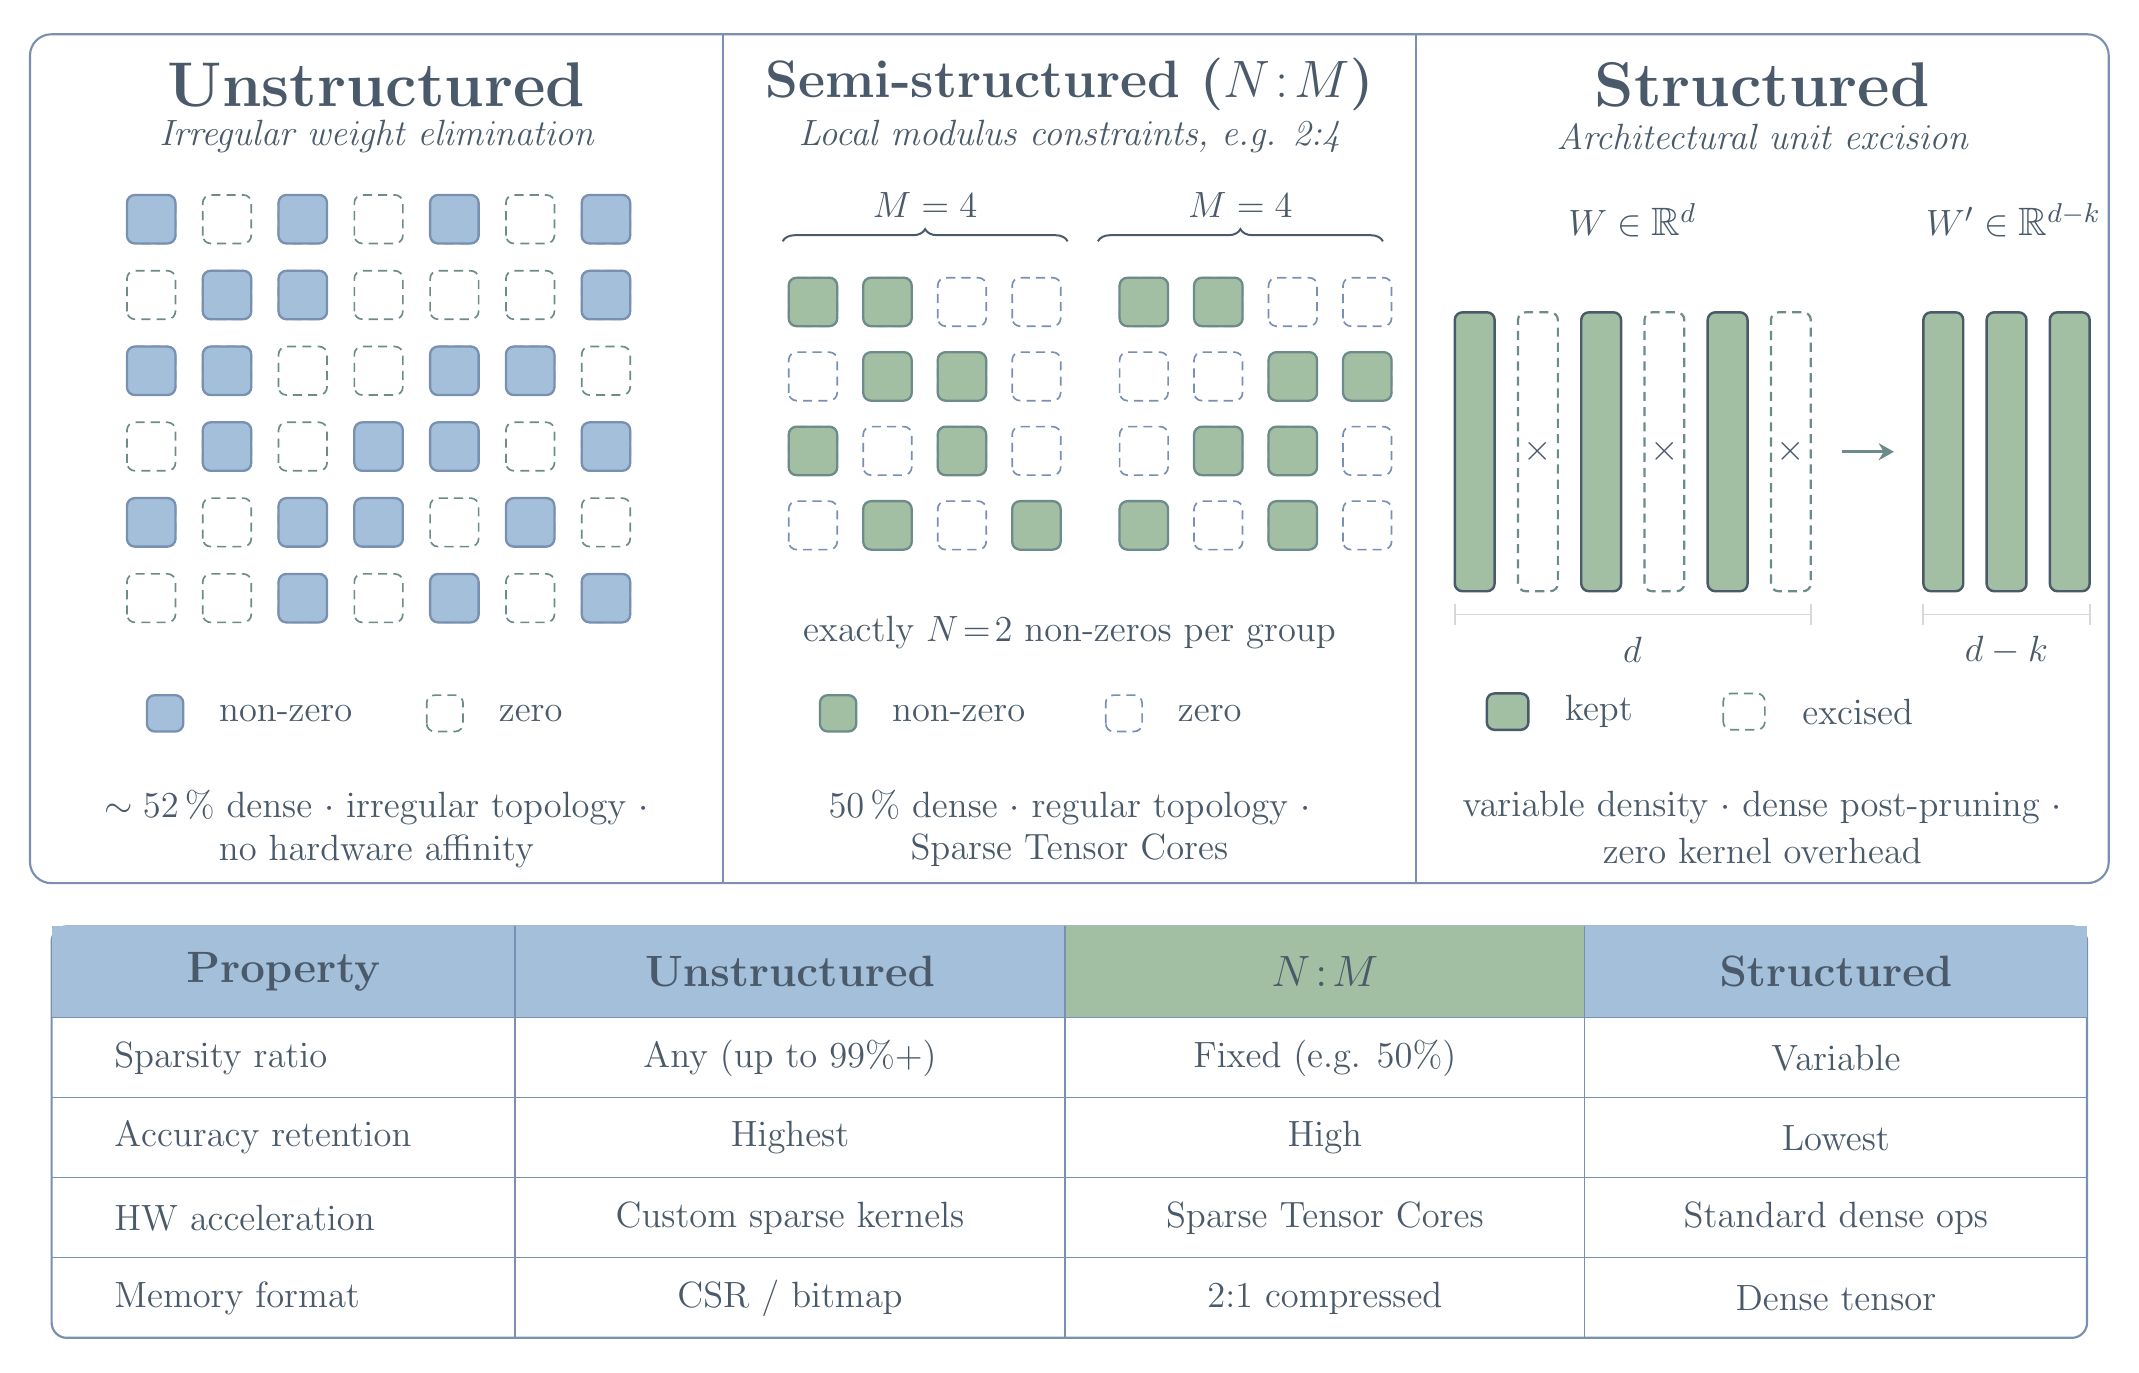
\includegraphics[width=0.72\textwidth]{figures/compression/pruning_s_ss_ns.PNG}
	\caption{Topologies of sparsity.}
	\label{fig:structures}
\end{figure}

\subsection{Semi-Structured Pruning ($N\!:\!M$ Sparsity)}

In \keyterm{$N\!:\!M$ sparsity}, weights are grouped into consecutive blocks
of $M$ elements, and exactly $N$ elements are retained in each block:
\begin{equation}
	\norm{m_\mathcal{G}}_0 = N \qquad \forall\,\mathcal{G},\;|\mathcal{G}|=M.
	\label{eq:nm_constraint}
\end{equation}
The 2:4 pattern ($N=2, M=4$) is the most important instance because NVIDIA's
Ampere and later architectures implement dedicated 2:4 sparse tensor-core
acceleration with a nominal $2\times$ throughput gain at 50\% sparsity
\cite{nvidia2020a100,mishra2021accelerating}.

The 2:4 sparse representation stores a \emph{compressed} weight matrix of
half the size plus a 2-bit index per retained element indicating its position
within its group.  The compression ratio is:
\begin{equation}
	\text{Storage}_{2:4} = \frac{N}{M}\,mn + \frac{N}{M}\,mn\,\frac{\log_2 M}{\text{bits/value}}.
\end{equation}
At FP16 with $M=4, N=2$: values take 16 bits each, indices take 2 bits each,
giving $16+2 = 18$ bits per retained weight versus 32 bits (FP16 for two
weights), achieving an approximately 1.78$\times$ compression in practice
rather than the theoretical $2\times$.

\subsection{Structured Pruning}

\keyterm{Structured pruning} removes whole vectors or submodules, yielding a
strictly smaller dense network with no irregular sparsity.  The removable unit
depends on the architecture:
Table \ref{tab:structured_units} summarises the common structured pruning units by architecture type, their effects on the model's topology, and their granularity.  Structured pruning is more amenable to hardware acceleration because it results in smaller dense operations that can be executed on standard BLAS/cuBLAS kernels without sparse indexing overhead.
\begin{table}[H]
	\centering
	\caption{Structured pruning units by architecture type.}
	\label{tab:structured_units}
	\renewcommand{\arraystretch}{1.4}
	\begin{tabularx}{\textwidth}{llXl}
		\toprule
		\textbf{Architecture} & \textbf{Unit} & \textbf{Effect} & \textbf{Granularity} \\
		\midrule
		MLP & Neuron (row + col) & Reduces hidden width & Fine \\
		CNN & Filter / channel & Reduces feature maps & Medium \\
		CNN & Convolutional block & Removes entire sub-network & Coarse \\
		Transformer & Attention head & Reduces attention diversity & Medium \\
		Transformer & FFN channel & Reduces intermediate width & Fine \\
		Transformer & Layer & Shortens depth & Very coarse \\
		Transformer & Token (dynamic) & Reduces sequence length & Input-dependent \\
		\bottomrule
	\end{tabularx}
\end{table}

%% ─────────────────────────────────────────────────────────────────────────
\section{Pruning Criteria}
\label{sec:pruning_criteria}
%% ─────────────────────────────────────────────────────────────────────────

A \keyterm{pruning criterion} assigns an importance score $S(\theta_i)$ (or
$S(g)$ for a structured group $g$) that serves as a proxy for the loss change
$\Delta\mathcal{L}$ induced by removing that element.  The ideal criterion
ranks units by \emph{true irreplaceability}: the unit with the lowest true
loss impact should be removed first.

\subsection{Magnitude-Based Criteria}

The most common zeroth-order criterion evaluates a weight by its absolute value:
\begin{equation}
	S_{\mathrm{mag}}(w_i) = |w_i|.
	\label{eq:mag}
\end{equation}
For structured groups (e.g.\ a convolutional filter
$W_g \in \R^{c_\mathrm{out} \times c_\mathrm{in} \times k \times k}$), the
criterion is extended via group norms:
\begin{align}
	S_g^{(1)} &= \norm{W_g}_1 = \sum_{i} |w_{g,i}|, \label{eq:mag_l1} \\
	S_g^{(2)} &= \norm{W_g}_2 = \sqrt{\sum_{i} w_{g,i}^2}, \label{eq:mag_l2} \\
	S_g^{(\infty)} &= \norm{W_g}_\infty = \max_i |w_{g,i}|. \label{eq:mag_linf}
\end{align}

The $\ell_2$ norm is the most common because it is differentiable and
rotation-invariant.  The $\ell_\infty$ norm is sensitive to outliers and
is less often used alone.

\textbf{Interpretation.} At a stationary point with a well-conditioned
Hessian, $S_{\mathrm{2nd}} = \tfrac{1}{2} H_{ii} w_i^2 \propto w_i^2$ if
$H_{ii}$ is approximately constant across parameters.  Under this assumption,
ranking by $|w_i|$ is equivalent to ranking by the second-order saliency.
When Hessian diagonal entries vary greatly across layers (which they do in
practice), magnitude alone may rank units from poorly-conditioned layers too
aggressively.

\subsection{Gradient-Based Criteria}

First-order saliency estimates include the effect of the local gradient \cite{molchanov2017variational}:
\begin{equation}
	S_{\mathrm{grad}}(w_i)
	= \left|\frac{\partial\mathcal{L}}{\partial w_i}\cdot w_i\right|.
	\label{eq:grad}
\end{equation}
This is obtained from the first-order Taylor term with $\delta w_i = -w_i$
(complete removal).  For structured pruning in Transformers the criterion is
extended to a head or FFN group by summing over all constituent parameters:
\begin{equation}
	S_{\mathrm{grad}}(g)
	= \left|\sum_{i \in g}\frac{\partial\mathcal{L}}{\partial w_i}\cdot w_i\right|.
	\label{eq:grad_group}
\end{equation}

\textbf{Movement pruning (Sanh et al.\ 2020).}  A related idea is to track
the \emph{movement} of weights from initialisation rather than their current
magnitude.  Score variables $v_i$ are trained alongside the network, and
the mask is derived from $v_i$ via a straight-through estimator.  This has
been shown to outperform magnitude pruning in fine-tuning regimes where
weights move substantially from pretraining.

\subsection{Second-Order Criteria}
\label{subsec:second_order_criteria}

\paragraph{Diagonal approximation (OBD style).}
\begin{equation}
	S_{\mathrm{2nd}}(w_i) = \frac{1}{2}\,H_{ii}\,w_i^2.
	\label{eq:second_order}
\end{equation}
$H_{ii}$ can be estimated from the Gauss-Newton approximation to the Hessian,
which requires computing per-sample gradients:
\begin{equation}
	H \approx G^\top G, \qquad G_{ij} = \frac{\partial \ell_j}{\partial w_i},
\end{equation}
where $\ell_j$ is the loss on sample $j$.  The diagonal is then
$H_{ii} \approx \sum_j G_{ij}^2$.

\paragraph{Blockwise inverse Hessian (SparseGPT style).}
For large linear layers, the exact per-weight OBS formula is applied
blockwise.  The layer weight matrix $W \in \R^{m \times n}$ is processed
column by column.  Let $\hat{H} = X X^\top / N$ be the empirical input
Hessian (second-moment matrix of activations), where
$X \in \R^{n \times N}$ contains $N$ calibration samples.  SparseGPT
\cite{frantar2023sparsegpt} prunes
one weight at a time from left to right, updating the remaining columns:
\begin{equation}
	W_{:,j}' = W_{:,j} - \frac{w_{:,j}}{[\hat{H}^{-1}]_{jj}}\, w_{:,j}^\top \hat{H}^{-1}_{j+1:, j},
	\label{eq:sparsegpt}
\end{equation}
then applying a Cholesky-based rank-1 update to $\hat{H}^{-1}$.  The total
cost is $O(n^3 + mn^2)$ per layer, which is tractable for Transformer FFN
layers ($n \approx 4096$).

\subsection{Activation-Aware Criteria}

Some methods compute saliency relative to the activation statistics the
weight processes.  The Wanda criterion uses activation-weighted magnitude
scores \cite{sun2023simple}:
\begin{equation}
	S_{\mathrm{act}}(W_{i,j}) = |W_{i,j}|\cdot\norm{x_j}_2,
	\label{eq:wanda}
\end{equation}
where $\norm{x_j}_2$ is the RMS activation magnitude of the $j$-th input
feature over a calibration set. This criterion reflects the fact that a small
weight attached to a consistently large input channel can contribute more to
the output than a larger weight attached to a weakly activated channel.

Large language models often exhibit pronounced \emph{outlier channels}, where
a small subset of feature dimensions has activation norms far above the
median \cite{wei2022outlier}. A magnitude-only rule treats weights attached to these channels as
equivalent to weights of the same size on ordinary channels, which can
underestimate their contribution. Activation-aware criteria such as Wanda
address this imbalance by rescaling importance according to input energy
\cite{sun2023simple}.

\subsection{Learnable and Adaptive Criteria}

A fourth family introduces \emph{trainable mask scores} $v \in \R^P$ that
are optimised jointly with weights:
\begin{equation}
	M_i = \sigma\!\left(\frac{v_i - \bar{v}}{\epsilon}\right),
	\quad
	\text{or}
	\quad
	M_i = \mathbf{1}[v_i \ge \tau],
	\label{eq:learnable}
\end{equation}
where the discrete threshold is approximated by a straight-through estimator
during backpropagation.  The learning objective includes a sparsity penalty:
\begin{equation}
	\mathcal{L}_{\mathrm{sparse}} = \mathcal{L}(\Theta, M(v)) + \lambda \norm{v}_1.
	\label{eq:learnable_loss}
\end{equation}

These methods are most useful when the training distribution is available and
the budget for mask optimisation is not a bottleneck.  They tend to
outperform static criteria at moderate sparsity levels in fine-tuning
settings.

\subsection{Criterion Comparison}
Table \ref{tab:criterion_comparison} summarises the information used for each criterion, the data needed to compute it, whether it requires gradients or Hessian information, and its typical accuracy relative to magnitude pruning.  Gradient-based and second-order criteria generally outperform magnitude pruning at the same sparsity, but they require additional data and computation.  Activation-aware criteria like Wanda can achieve strong post-training performance without gradients or Hessians by leveraging activation statistics.  Learnable criteria offer the best accuracy when fine-tuning is possible but are less practical for one-shot pruning of frozen models.
\begin{table}[H]
	\centering
	\caption{Summary comparison of pruning criteria.}
	\label{tab:criterion_comparison}
	\renewcommand{\arraystretch}{1.5}
	\begin{tabularx}{\textwidth}{lXXccl}
		\toprule
		\textbf{Criterion} & \textbf{Information used}
		& \textbf{Data needed}
		& \textbf{Grad?} & \textbf{$H$?}
		& \textbf{Typical accuracy} \\
		\midrule
		Magnitude & Weight values only
		& None & No & No & Baseline \\
		Gradient (Taylor) & Gradient $\times$ weight
		& Train/calib & Yes & No & +1--3\% over mag \\
		OBD & Diag.\ curvature
		& Train/calib & Yes & Diag & +1--5\% over mag \\
		OBS / SparseGPT & Full curvature per layer
		& Calibration & No & Block & Best (post-train) \\
		Wanda & Magnitude $\times$ activation
		& Calibration & No & No & Strong post-train \\
		Movement & Score trajectory
		& Fine-tune & Yes & No & Best for fine-tune \\
		\bottomrule
	\end{tabularx}
\end{table}

%% ─────────────────────────────────────────────────────────────────────────
\section{Pruning Strategies}
%% ─────────────────────────────────────────────────────────────────────────

A \keyterm{pruning strategy} specifies \emph{when}, \emph{how often}, and
\emph{in what order} the criterion is evaluated and the mask is updated over
time.  Strategy choice is largely orthogonal to criterion choice.

\subsection{One-Shot Pruning}

In \keyterm{one-shot pruning} (also called single-step pruning), the importance
scores are computed once using the fully trained model, and all pruning
decisions are made in a single pass:

%\begin{algorithm}[H]
%	\SetAlgoLined
%	\KwIn{Trained model $f(\cdot;\Theta)$, target density $\kappa$}
%	\KwOut{Pruned model $f(\cdot; M \odot \Theta)$}
%	Compute $S(\theta_i)$ for all $i \in [P]$\;
%	Set threshold $\tau \leftarrow$ $(1-\kappa)$ quantile of $\{S(\theta_i)\}$\;
%	$M_i \leftarrow \mathbf{1}[S(\theta_i) \ge \tau]$\;
%	\textbf{Optional:} fine-tune $\Theta$ with $M$ fixed\;
%	\Return $M \odot \Theta$\;
%	\caption{One-Shot Pruning}
%	\label{alg:one_shot}
%\end{algorithm}

The algorithm is straightforward: compute scores, determine the threshold for the desired density, and apply the mask.  Optionally, a short fine-tuning phase can be added after pruning to recover some accuracy.

\textbf{Advantages:}  Computationally cheap; no multiple rounds of
training; directly applicable to frozen pretrained models.

\textbf{Disadvantages:}  All decisions are made from one snapshot of the
loss landscape; errors compound without correction; typically yields lower
accuracy than iterative methods at the same sparsity.

\subsection{Iterative Pruning and Recovery}
\label{subsec:iterative_pruning}

\keyterm{Iterative pruning} interleaves mask updates with weight recovery
(fine-tuning or retraining):

%\begin{algorithm}[H]
%	\SetAlgoLined
%	\KwIn{Trained model $\Theta$, target density $\kappa$, rounds $R$}
%	\KwOut{Pruned model $M \odot \Theta$}
%	$\kappa_0 \leftarrow 1.0$\;
%	\For{$r = 1$ \KwTo $R$}{
%		$\kappa_r \leftarrow \kappa + (1 - \kappa)\left(1 - \tfrac{r}{R}\right)^3$
%		\quad\textit{// cubic sparsity schedule}\;
%		Compute scores $S(\theta_i)$ on current $\Theta$\;
%		Update mask $M$ to density $\kappa_r$\;
%		Fine-tune $\Theta$ with $M$ fixed for $T_r$ steps\;
%	}
%	\Return $M \odot \Theta$\;
%	\caption{Iterative Pruning with Cubic Schedule}
%	\label{alg:iterative}
%\end{algorithm}

The algorithm proceeds in $R$ rounds.  In each round, the target density $\kappa_r$ is updated according to a schedule, scores are recomputed on the current model, the mask is updated to the new density, and the model is fine-tuned to recover from pruning-induced loss increases.  The schedule $\kappa_r$ controls how aggressively pruning is applied in each round.  A common choice is a cubic schedule:
\begin{equation}
	\kappa_r = \kappa + (1 - \kappa)\left(1 - \frac{r}{R}\right)^3,
\end{equation}
which front-loads pruning by removing most redundancy early and reserving few rounds for fine-grained refinement near the target density.  This allows the model to stabilise as it approaches the final sparsity level, which can improve accuracy compared to a linear schedule that prunes at a constant rate.
The cubic schedule $\kappa_r = \kappa + (1-\kappa)(1 - r/R)^3$ front-loads
pruning, removing most redundancy early and reserving few rounds for
fine-grained refinement near the target density.

%\begin{figure}[H]
%	\centering
%	\begin{tikzpicture}
%		\begin{axis}[
%			width=0.92\linewidth, height=5.5cm,
%			xlabel={Round ($r/R$)},
%			ylabel={Sparsity $s_r$ (\%)},
%			xmin=0, xmax=1, ymin=0, ymax=95,
%			legend pos=south east,
%			legend style={font=\small},
%			grid=both, grid style={gray!15},
%			xtick={0,0.25,0.5,0.75,1.0},
%			ytick={0,20,40,60,80,90},
%			title={Sparsity Schedules for Iterative Pruning ($\kappa = 0.10$)},
%			title style={font=\small\bfseries},
%			]
%			% Linear schedule
%			\addplot[very thick, colBlueBorder, domain=0:1, samples=50]
%			{90 * x};
%			\addlegendentry{Linear}
%
%			% Cubic schedule (front-loaded)
%			\addplot[very thick, headergreen, domain=0:1, samples=50]
%			{90 * (1 - (1-x)^3)};
%			\addlegendentry{Cubic (front-loaded)}
%
%			% Step schedule
%			\addplot[very thick, actreddark, const plot]
%			coordinates {(0,0)(0.2,30)(0.4,60)(0.6,75)(0.8,85)(0.9,90)(1,90)};
%			\addlegendentry{Step}
%
%			% Cosine schedule
%			\addplot[very thick, slateblue, domain=0:1, samples=50]
%			{90 * 0.5 * (1 - cos(deg(pi * x)))};
%			\addlegendentry{Cosine}
%		\end{axis}
%	\end{tikzpicture}
%	\caption{Illustration of different sparsity schedules for iterative pruning
%		targeting 90\% sparsity over $R$ rounds.  Cubic and cosine schedules are
%		generally preferred as they allow the model to stabilise near the target
%		sparsity before the final mask is frozen.}
%	\label{fig:schedules}
%\end{figure}

\subsection{Pruning During Training}

Some methods integrate sparsity discovery directly into the optimisation loop:

\begin{itemize}
	\item \textbf{Dynamic sparse training (DST):}  Periodically drops the
	lowest-scoring active weights and revives the highest-scoring pruned
	weights, maintaining a fixed sparsity level throughout.
	\item \textbf{Regularisation-based:}  Adds an $\ell_1$ penalty
	$\lambda \sum_i |\theta_i|$ to the loss, encouraging sparsity; weights
	near zero are later hard-thresholded.
	\item \textbf{Variational dropout:}  Places log-uniform priors on weights,
	leading each weight to learn its own noise level; high noise implies the
	weight can safely be pruned.
\end{itemize}

\subsection{Post-Training Pruning}
\label{sec:post_training_pruning}

\keyterm{Post-training pruning (PTP)} applies pruning to a frozen pretrained
model using only a small calibration set, without repeating full training.
This regime is especially relevant for very large models ($\ge 7$B parameters),
where full retraining is operationally expensive. The general pipeline is:

\begin{figure}[H]
	\centering
	\begin{adjustbox}{max width=\linewidth}
	\begin{tikzpicture}[
		font=\small,
		box/.style={rectangle, rounded corners=3pt, draw=colBlueBorder, fill=colBlue!15,
			minimum width=2.8cm, minimum height=0.7cm, align=center},
		data/.style={rectangle, rounded corners=3pt, draw=headergreen, fill=colGreen!25,
			minimum width=2.8cm, minimum height=0.7cm, align=center},
		arr/.style={-Stealth, thick, colBlueBorder}
		]
		\node[data]  (pretrain)   {Pretrained\\$\Theta^*$};
		\node[data, right=0.8cm of pretrain] (calib)
		{Calibration\\data ($\le$512 samples)};
		\node[box, right=0.8cm of calib]  (stats)
		{Compute\\activation\\statistics};
		\node[box, right=0.8cm of stats]  (score)
		{Score each\\weight/group\\$S(\theta_i)$};
		\node[box, right=0.8cm of score]  (mask)
		{Apply mask\\$M^*$};
		\node[box, right=0.8cm of mask]   (opt)
		{(Optional)\\Weight\\correction};
		\node[data, below=0.7cm of opt]   (pruned)
		{Pruned model\\$M^* \odot \Theta^*$};
		
		\draw[arr] (pretrain) -- (stats);
		\draw[arr] (calib)    -- (stats);
		\draw[arr] (stats)    -- (score);
		\draw[arr] (score)    -- (mask);
		\draw[arr] (mask)     -- (opt);
		\draw[arr] (opt)      -- (pruned);
	\end{tikzpicture}
	\end{adjustbox}
	\caption{Post-training pruning pipeline.  No gradient update to the original
		pretraining loss is required; only calibration statistics and optional
		local weight corrections (as in SparseGPT) are needed.}
	\label{fig:ptp_pipeline}
\end{figure}

\subsection{Global vs.\ Layerwise Allocation}

A critical strategic decision is how the sparsity budget $\kappa$ is
distributed across layers.

\paragraph{Layerwise allocation.} Assign the same target density $\kappa$ to
every layer.  Simple but suboptimal: sensitive layers (usually the first,
last, and attention output projections) are pruned as aggressively as
insensitive ones.

\paragraph{Global allocation.} Pool all parameters and rank them by a
normalised importance score across the entire network.  Let the global
score for parameter $i$ in layer $l$ be:
\begin{equation}
	S_i^{\mathrm{global}} = \frac{S_i^{(l)}}{\max_{j \in l} S_j^{(l)}},
	\label{eq:global_score}
\end{equation}
then apply a single threshold $\tau$ across all layers.  This allows some
layers to be nearly dense while others are very sparse.

\paragraph{Sensitivity-guided allocation.}  Profile the loss sensitivity of
each layer by measuring the increase in validation loss when that layer is
independently pruned to various densities.  Use these profiles to set
per-layer targets $\kappa_l$ that equalise the marginal loss impact:
\begin{equation}
	\frac{\partial \mathcal{L}_{\mathrm{val}}}{\partial s_l}
	= \text{const} \quad \forall\,l.
	\label{eq:sensitivity}
\end{equation}

Figure~\ref{fig:layer_sensitivity} conceptually illustrates layer-wise
sensitivity in a Transformer.

\begin{figure}[H]
	\centering
	\begin{tikzpicture}
		\begin{axis}[
			ybar, bar width=10pt,
			width=0.92\linewidth, height=5.5cm,
			xlabel={Layer index},
			ylabel={Loss increase at 50\% sparsity},
			xtick={1,...,12},
			xticklabels={1,2,3,4,5,6,7,8,9,10,11,12},
			ymin=0, ymax=0.25,
			ymajorgrids=true, grid style={gray!20},
			title={Conceptual Per-Layer Sensitivity (12-layer Transformer)},
			title style={font=\small\bfseries},
			legend pos=north west,
			]
			\addplot[fill=actred, draw=actreddark] coordinates {
				(1,0.19)(2,0.06)(3,0.04)(4,0.05)(5,0.03)(6,0.04)
				(7,0.05)(8,0.04)(9,0.06)(10,0.08)(11,0.12)(12,0.22)
			};
			\addlegendentry{Attention}
			\addplot[fill=colBlue!75!white, draw=colBlueBorder] coordinates {
				(1,0.12)(2,0.04)(3,0.03)(4,0.03)(5,0.02)(6,0.03)
				(7,0.03)(8,0.03)(9,0.04)(10,0.05)(11,0.09)(12,0.14)
			};
			\addlegendentry{FFN}
		\end{axis}
	\end{tikzpicture}
	\caption{Conceptual illustration of per-layer loss sensitivity in a 12-layer
		Transformer at 50\% sparsity.  First and last layers are typically most
		sensitive.  An optimal allocation should assign higher density to high
		sensitivity layers.}
	\label{fig:layer_sensitivity}
\end{figure}

%% ─────────────────────────────────────────────────────────────────────────
\section{Pruning Transformers}
%% ─────────────────────────────────────────────────────────────────────────

In transformers, we have the same objective of removing parameters while preserving the loss, formalised as in the general pruning problem \eqref{eq:constrained}:
\begin{equation}
	\min_{M \in \{0,1\}^P} \mathcal{L}(M \odot \Theta) \quad \text{subject to} \norm{M}_0 \le \kappa P.
	\label{eq:transformer_pruning}
\end{equation}
Transformer pruning requires special treatment because the main computational
units are not simple neurons or filters.  The most common removable structures
are attention heads, FFN intermediate channels, entire layers, and (in some
settings) tokens.

\subsection{Attention Head Pruning}

A head mask $m \in \{0,1\}^H$ zeros out entire heads from the concatenation:
\begin{equation}
	\mathrm{MHA}_m(X) = \mathrm{Concat}(m_1\,\mathrm{head}_1(X), \ldots,
	m_H\,\mathrm{head}_H(X))\,W_O.
	\label{eq:mha_masked}
\end{equation}
Setting $m_h = 0$ zeroes four weight matrices:
$W_{Q_h}, W_{K_h}, W_{V_h} \in \R^{d \times d_h}$ and the corresponding
columns of $W_O \in \R^{d \times d}$.  Total parameters removed per head:
\begin{equation}
	\Delta P_{\mathrm{head}} = 4\,d\,d_h = 4\,d\,\frac{d}{H} = \frac{4d^2}{H}.
	\label{eq:head_params}
\end{equation}
For GPT-2 ($d=768, H=12$): removing one head removes
$4 \times 768 \times 64 = 196{,}608$ parameters ($\approx 0.18\%$ of the
full model).

\paragraph{Empirical findings.} Empirical studies consistently report the
following patterns:
\begin{itemize}
	\item Many models can operate with 20--40\% of heads removed without
	statistically significant performance loss.
	\item Some heads perform identifiable \emph{linguistic functions}
	(positional, coreference, syntactic), making them harder to remove.
	\item The importance of a head varies greatly by layer; earlier and later
	layers tend to be more sensitive than middle layers.
\end{itemize}

\subsection{FFN Channel Pruning}

An FFN channel mask $g \in \{0,1\}^{rd}$ selects which intermediate neurons
to retain:
\begin{equation}
	\mathrm{FFN}_g(X) = \phi(XW_1 + b_1)\,\diag(g)\,W_2 + b_2.
	\label{eq:ffn_masked}
\end{equation}
Let $\mathcal{K} = \{k : g_k = 1\}$.  Then in compact form:
\begin{equation}
	\mathrm{FFN}_g(X) = \phi(X W_{1,\mathcal{K}} + b_{1,\mathcal{K}})\,W_{2,\mathcal{K},:} + b_2.
	\label{eq:ffn_compact}
\end{equation}
This is a dense computation with intermediate dimension $|\mathcal{K}| \le rd$.
Parameters removed: $(2d) \times (rd - |\mathcal{K}|)$ (rows of $W_1$ plus
columns of $W_2$).

In modern LLMs using SwiGLU activations:
\begin{equation}
	\mathrm{FFN}_{\mathrm{SwiGLU}}(X) = \bigl(\sigma(XW_{\mathrm{gate}}) \cdot XW_1\bigr)W_2,
	\label{eq:swiglu}
\end{equation}
FFN pruning must jointly mask corresponding channels of $W_{\mathrm{gate}}$,
$W_1$, and $W_2$ since the gate and linear branches are entangled.

\subsection{Layer Pruning}

Layer pruning removes entire Transformer blocks. A common formulation
treats each block as a residual function $x \mapsto x + F_l(x)$ and measures
the block's contribution as the normalised distance:
\begin{equation}
	S_l^{\mathrm{block}} = \frac{\norm{F_l(X)}_F}{\norm{X}_F},
	\label{eq:block_sensitivity}
\end{equation}
estimated over calibration samples.  Blocks with very small angular change
(nearly identity function) can be removed with negligible effect on outputs.

Layer pruning drastically reduces depth-dependent inference latency (which
scales as $O(L \cdot d^2)$ for $L$ layers) but also reduces model capacity
substantially.  At aggressive layer-pruning ratios ($> 30\%$), perplexity
typically degrades significantly and fine-tuning recovery is necessary.

\subsection{Token Pruning}

Token pruning is unique in that it is \emph{input-dependent}: the number and
identity of pruned tokens changes for each sequence. It relies on the
observation that not all tokens require full attention computation at every
layer. An
importance score is computed per token:
\begin{equation}
	S_t = \sum_{h=1}^{H} \sum_{t'=1}^{T} A_{h,t,t'},
	\label{eq:token_score}
\end{equation}
where $A_{h,t,t'}$ is the attention weight from query $t$ to key $t'$ in head
$h$.  Tokens receiving low total attention are candidates for early exit or
pooling.

Token pruning is especially relevant for long-context inference where the
$O(T^2)$ attention cost dominates.  Methods such as $H_2O$ (Heavy-Hitter
Oracle) and StreamingLLM exploit the observation that a small fraction of
\emph{heavy-hitter} tokens accumulate disproportionate attention mass.

\section{Conclusion}

This chapter established the conceptual and mathematical foundations of neural
network pruning. It formalized pruning as a constrained optimization problem,
introduced the main structural sparsity regimes, and compared the principal
criteria used to estimate removal saliency, from magnitude-based and
gradient-based rules to activation-aware and second-order formulations.

\noindent The chapter also distinguished between pruning strategies, including
one-shot, iterative, training-time, and post-training regimes, and examined the
specific structures that make Transformer pruning distinct, particularly
attention heads, FFN channels, layers, and tokens. These foundations motivate
the method-level review in Chapter~\ref{chap:related_work_pruning}, where pruning approaches are
compared according to their optimization signals, recovery requirements, and
deployment objectives.

\noindent These foundations also establish the terms in which pruning methods
should be compared. Differences in sparsity topology, pruning unit, saliency
signal, recovery procedure, and deployment objective are not secondary
implementation details; they correspond to distinct problem settings. The
literature review that follows is organized along precisely these dimensions.
